\section{安装Storm}
\subsection{简介}
Storm是一款实时流处理框架,以实时性为特点,其延迟比Spark Streaming还要低,为毫秒级。多与Kafka等工具结合起来使用。
其安装配置需要搭配Zookeeper进行。

Hadoop、Sqark和Storm是Apache基金会的三个顶级项目。Storm与Hadoop相比的特点主要是流式计算,而
Hadoop是批处理作业。Storm的运行可以没有HDFS,只要有Zookeeper就可以,但是Storm也可以
和HDFS交互,也属于生态系统重要组成。

Storm的核心组件:

\begin{itemize}
	\item Nimbus:即Storm的Master,负责资源分配和任务调度。一个Storm集群只有一个Nimbus。
	\item Supervisor:即Storm的Slave,负责接收Nimbus分配的任务,管理所有Worker,一个Supervisor节点中包含多个Worker进程。
	\item Worker:工作进程,每个工作进程中都有多个Task。
	\item Task:任务,在 Storm 集群中每个 Spout 和 Bolt 都由若干个任务(tasks)来执行。每个任务都与一个执行线程相对应。
	\item Topology:计算拓扑,Storm 的拓扑是对实时计算应用逻辑的封装,它的作用与 MapReduce 的任务(Job)很相似,区别在于 MapReduce 的一个 Job 在得到结果之后总会结束,而拓扑会一直在集群中运行,直到你手动去终止它。拓扑还可以理解成由一系列通过数据流(Stream Grouping)相互关联的 Spout 和 Bolt 组成的的拓扑结构。
	\item Stream:数据流(Streams)是 Storm 中最核心的抽象概念。一个数据流指的是在分布式环境中并行创建、处理的一组元组(tuple)的无界序列。数据流可以由一种能够表述数据流中元组的域(fields)的模式来定义。
	\item Spout:数据源(Spout)是拓扑中数据流的来源。一般 Spout 会从一个外部的数据源读取元组然后将他们发送到拓扑中。根据需求的不同,Spout 既可以定义为可靠的数据源,也可以定义为不可靠的数据源。一个可靠的 Spout能够在它发送的元组处理失败时重新发送该元组,以确保所有的元组都能得到正确的处理;相对应的,不可靠的 Spout 就不会在元组发送之后对元组进行任何其他的处理。一个 Spout可以发送多个数据流。
	\item Bolt:拓扑中所有的数据处理均是由 Bolt 完成的。通过数据过滤(filtering)、函数处理(functions)、聚合(aggregations)、联结(joins)、数据库交互等功能,Bolt 几乎能够完成任何一种数据处理需求。一个 Bolt 可以实现简单的数据流转换,而更复杂的数据流变换通常需要使用多个 Bolt 并通过多个步骤完成。
	\item Stream grouping:为拓扑中的每个 Bolt 的确定输入数据流是定义一个拓扑的重要环节。数据流分组定义了在 Bolt 的不同任务(tasks)中划分数据流的方式。在 Storm 中有八种内置的数据流分组方式。
	\item Reliability:可靠性。Storm 可以通过拓扑来确保每个发送的元组都能得到正确处理。通过跟踪由 Spout 发出的每个元组构成的元组树可以确定元组是否已经完成处理。每个拓扑都有一个“消息延时”参数,如果 Storm 在延时时间内没有检测到元组是否处理完成,就会将该元组标记为处理失败,并会在稍后重新发送该元组。
\end{itemize}

\subsection{安装配置}

首先需要修改\lstinline{storm-env.sh}文件和\lstinline{storm_env.ini}文件。
\lstinputlisting[style=mysh,title=storm-env.sh]{docs/storm/conf/storm-env.sh}

\lstinputlisting[style=mysh,title=storm\_env.ini]{docs/storm/conf/storm_env.ini}

在其中主要配置的是Java运行环境。更多的配置更主要需要修改\lstinline{storm.yaml}文件。

\lstinputlisting[style=mysh,title=storm.yaml]{docs/storm/conf/storm.yaml}

\begin{itemize}
    \item \lstinline{storm.zookeeper.servers}配置的是ZK服务的集群。这里就填入配置好的ZK集群地址,ZK集群的配置可以见上面。
    \item \lstinline{nimbus.seeds}是有机会成为活跃\lstinline{nimbus}的机器。
    \item \lstinline{ui.port}原来的UI端口是8080,这里使用时总是出现端口占用的情况,因此指定为9090。
    \item \lstinline{supervisor.slots.ports}这个指定的是supervisor运行时slots可用的端口。这里采用的是官网上推荐的默认配置,指定了4个,表明最大会有4个Worker进程在一台机器上运行,具体的Worker数量,可以在代码中指定。
    \item \lstinline{storm.local.dir},本地存储数据目录,需要提前创建。
    \item \lstinline{storm.health.check.dir},存储健康检测信息目录。
    \item \lstinline{storm.health.check.timeout.ms},健康检测时长。
    \item \lstinline{drpc.servers}。DRPC(Distribuition Remote Process Call)分布式远程过程调用服务,指定服务地址。
\end{itemize}

\subsection{测试和运用}
启动安装配置好后可以启动Storm。
启动顺序如下:

\lstinputlisting[style=mysh,title=start-storm.sh启动storm的顺序]{docs/storm/start-storm.sh}

注意上面的命令加了\lstinline{&},指定其进程在后台运行。
需要在不同的节点上都启动,但是活跃的Nimbus只有一个,这个由ZK完成选取。
启动后可以在Web浏览器9090(依据上面配置)查看Storm UI,启动了LogViewer,可以在8000端口查看各个Nimbus和Supervisor的
日志信息。

\begin{center}
    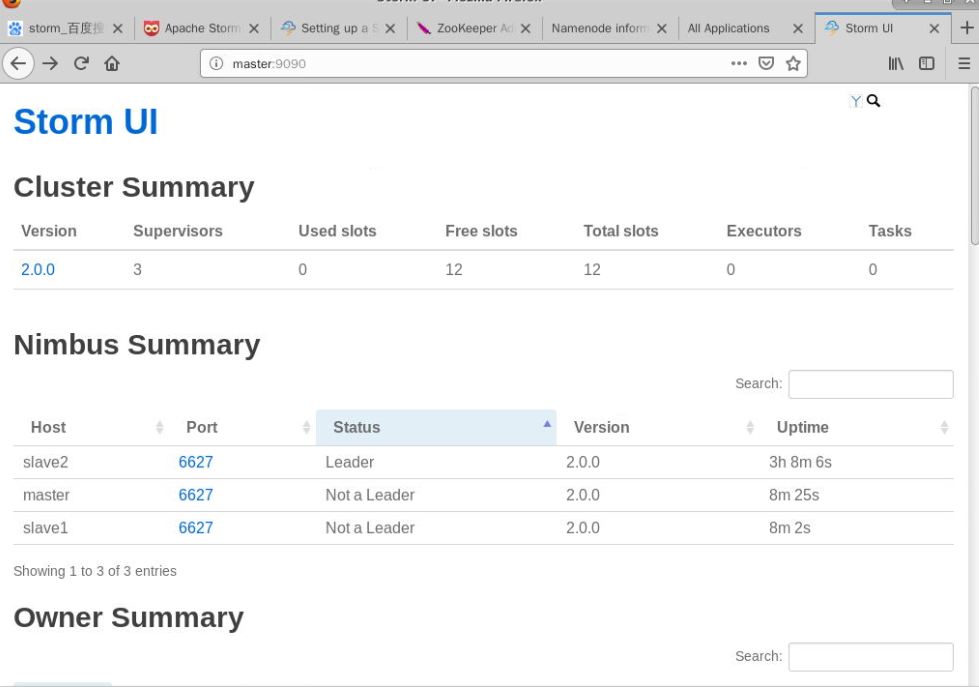
\includegraphics[width=\linewidth]{storm/stormui1.png}

    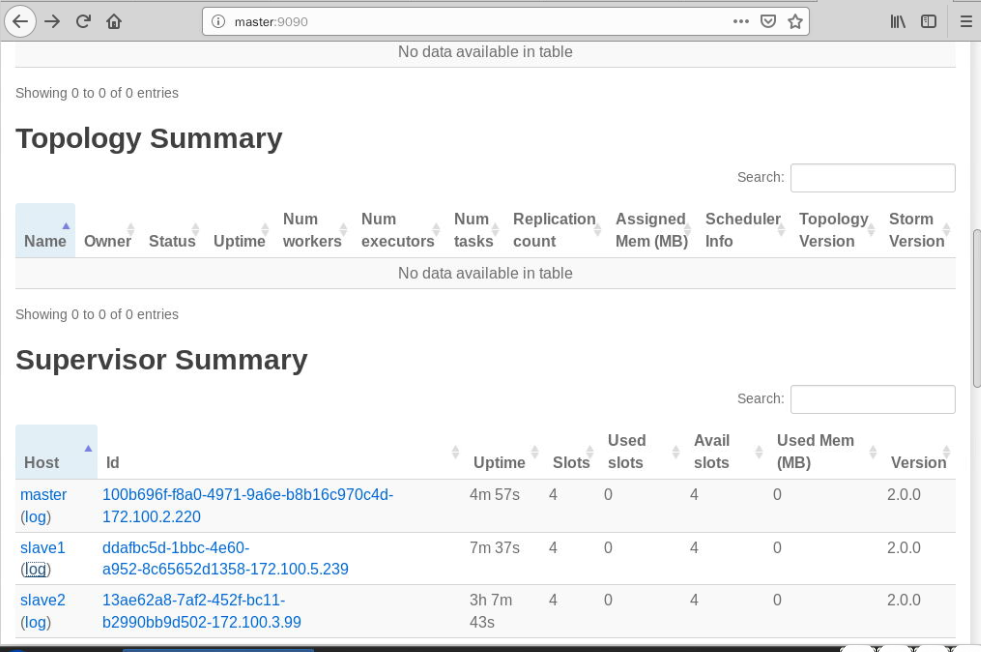
\includegraphics[width=\linewidth]{storm/stormui2.png}

    Storm UI上查看很多集群相关有用的信息
\end{center}

\begin{center}
    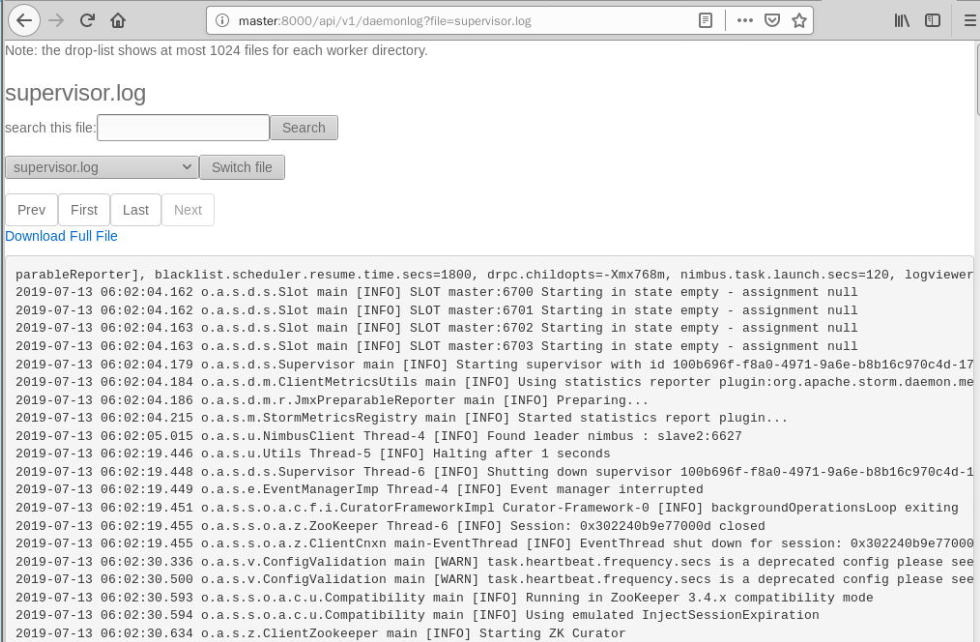
\includegraphics[width=\linewidth]{storm/logviewer.png}

    点击log查看各个节点的log信息,需要启动logviewer服务
\end{center}

\subsection{Java编程实例}

Storm以实时流计算为特色,能够在很大程度上弥补MapReduce作业在实时性上的缺点和不足。
利用Storm提供的Java API,可以自定义数据源Spout和数据处理点Bolt。下面分析是一个利用
Storm官方提供的Word Count Example编写的WordCount例子。

编写Storm程序,主要需要定义Spout、Bolt和Topology。
Spout的定义一般是实现\lstinline{IRichSpout}接口或继承\lstinline{BaseRichSpout}类。
对应Bolt类一般是实现\lstinline{IRichBolt}接口或继承\lstinline{BaseRichBolt}类。
两种都是可以的,后者更为简单一些,是对前者的一层封装。

下面是用于随机生成句子的Spout类:

\lstinputlisting[style=customjava,title=RandomSentenceSpout.java]{docs/storm/RandomSentenceSpout.java}

\begin{lstlisting}[style=customjava]
@Override
public void nextTuple() {
	String[] sentences = new String[]{
			sentence("the cow jumped over the moon"), sentence("an apple a day keeps the doctor away"),
			sentence("four score and seven years ago"), sentence("snow white and the seven dwarfs"), sentence("i am at two with nature")
	};
	final String sentence = sentences[rand.nextInt(sentences.length)];

	LOG.debug("Emitting tuple: {}", sentence);

	collector.emit(new Values(sentence));
}	
\end{lstlisting}

\lstinline{nextTuple()}是其中处理业务的核心方法。该方法会被放在一个无限运行的循环中,不断地通过\lstinline{emit}
发送出数据,就像是“水龙头”一样。这也是Storm与MapReduce程序的区别,在定义好拓扑后,Storm是不断运行的。

其他几个必须要实现的方法中(主要继承至\lstinline{IRichSout})分别有对应的功能。

下面是定义拓扑结构的类以及两个处理节点\lstinline{SplitSentence}和\lstinline{WordCount}
都简单起见作为静态类写在了内部,分别用来将句子分割为单词串和将
单词进行词频统计。

\lstinputlisting[style=customjava,title=WordCountApp.java]{docs/storm/WordCountApp.java}


\lstinline{execute}是实现Bolt逻辑的主要方法,\lstinline{prepare}用于在处理之前做一些准备,\lstinline{declareOutputFields}
声明输出的\lstinline{Field}。

\begin{lstlisting}[style=customjava]
// 将句子进行分词
@Override
public void execute(Tuple input) {
	String sentence = input.getStringByField("word");
	String[]  words = sentence.split(" ");
	for(String word: words) {
		this.collector.emit(new Values(word));
	}
}
// 实现统计词频
@Override
public void execute(Tuple tuple, BasicOutputCollector collector) {
	String word = tuple.getString(0);
	Integer count = counts.get(word);
	if (count == null) {
		count = 0;
	}
	count++;
	counts.put(word, count);
	collector.emit(new Values(word, count));
}
\end{lstlisting}

注意里面设置了集群模式提交和本地模式运行的判断:

\begin{lstlisting}[style=customjava]
if (args != null && args.length > 0) {
	topologyName = args[0];
	StormSubmitter.submitTopology(topologyName, conf, builder.createTopology());
} else {
	LocalCluster cluster = new LocalCluster();
	cluster.submitTopology(topologyName, conf, builder.createTopology());
	Thread.sleep(1000 * waitTime);
	cluster.killTopology(topologyName);
	cluster.shutdown();
}	
\end{lstlisting}

本地模式需要设置运行的结束时间,在这里不是无限循环运行的。

下面代码用于设置拓扑结构、分组策略以及并发程度,这些会影响作业的执行情况。
\begin{lstlisting}[style=customjava]
TopologyBuilder builder = new TopologyBuilder();
builder.setSpout("spout", new RandomSentenceSpout(), 3);
builder.setBolt("split", new SplitSentence(), 8).shuffleGrouping("spout");
builder.setBolt("count", new WordCount(), 12).fieldsGrouping("split", new Fields("word"));
\end{lstlisting}

在本地运行的结果如下:

\begin{figure}[h]
	\centering
	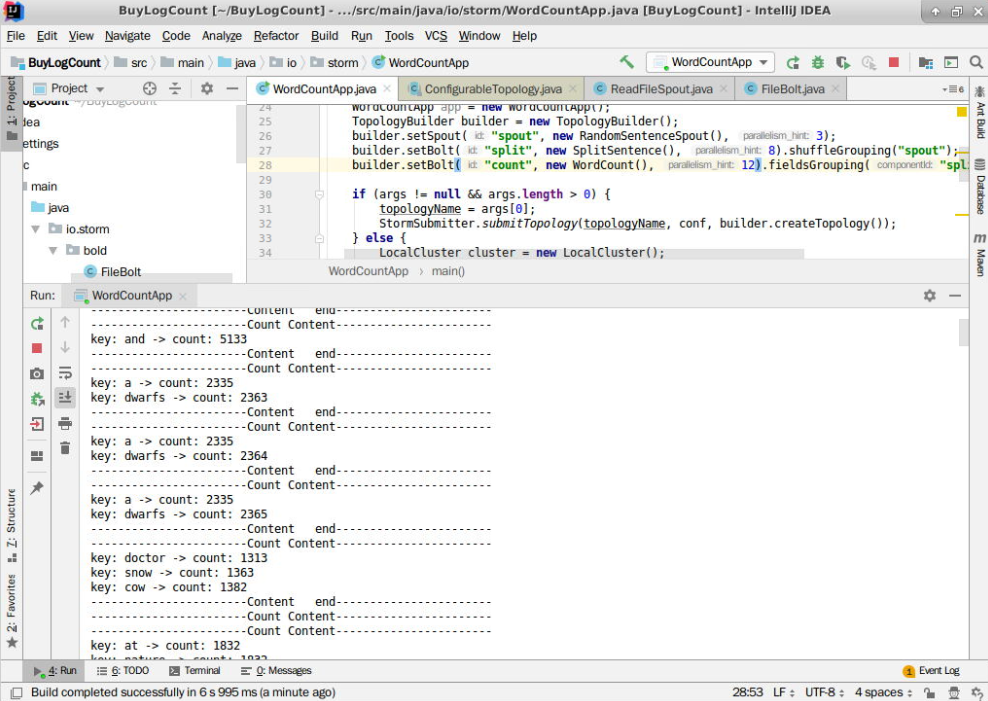
\includegraphics[width=\linewidth]{storm/runlocal.png}
	\caption{词频统计程序本地运行情况}
	\label{fig:storm-run-local}
\end{figure}

还可以通过下面命令将Jar包提交到集群中进行运行。

\lstinputlisting[style=mysh,title=提交Storm集群Jar包的命令]{docs/storm/use-storm.sh}

提交集群运行后,可以在UI界面中查看相关拓扑运行情况。

\begin{figure}[h]
	\centering
	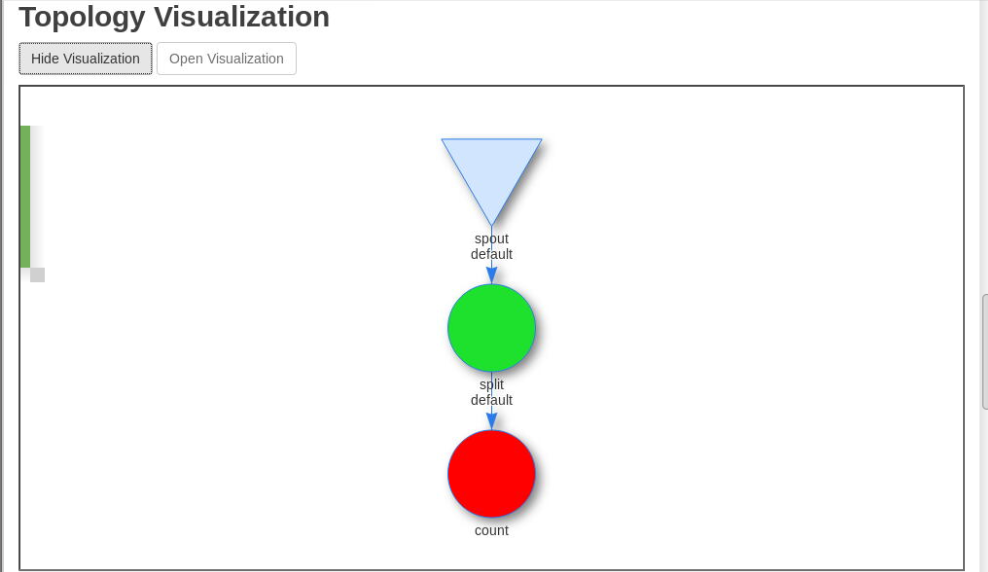
\includegraphics[width=0.8\linewidth]{storm/topoview.png}
	\caption{查看可视化拓扑结构,该例子比较简单,只有一个Spout和两个顺序的Bolt}
\end{figure}

\begin{center}
	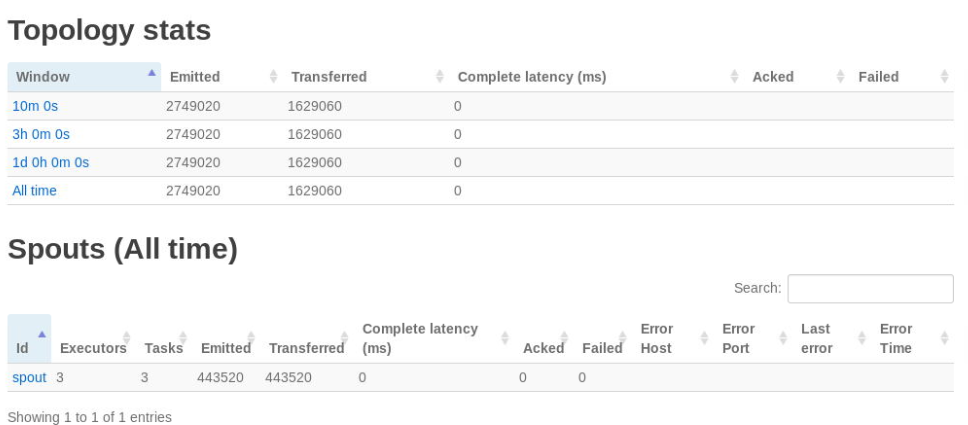
\includegraphics[width=\linewidth]{storm/topostat.png}

	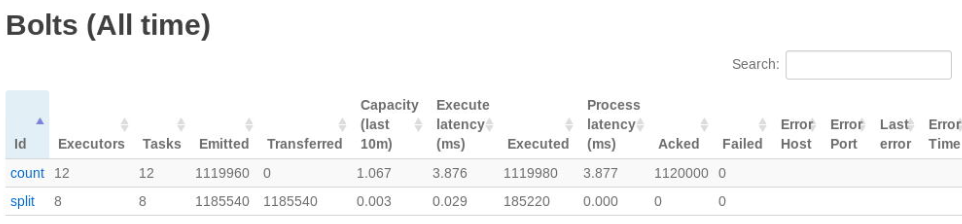
\includegraphics[width=\linewidth]{storm/bolts.png}

	查看拓扑运行Worker进程、数据压力等统计信息
\end{center}
